%%%%%%%%%%%%%%%%%%%%%%%%%%%%%%%%%%%%%%%%%
% University Assignment Title Page
% LaTeX Template
% Version 1.0 (27/12/12)
%
% This template has been downloaded from:
% http://www.LaTeXTemplates.com
%
% Original author:
% WikiBooks (http://en.wikibooks.org/wiki/LaTeX/Title_Creation)
%
% License:
% CC BY-NC-SA 3.0 (http://creativecommons.org/licenses/by-nc-sa/3.0/)
%
% Instructions for using this template:
% This title page is capable of being compiled as is. This is not useful for
% including it in another document. To do this, you have two options:
%
% 1) Copy/paste everything between \begin{document} and \end{document}
% starting at \begin{titlepage} and paste this into another LaTeX file where you
% want your title page.
% OR
% 2) Remove everything outside the \begin{titlepage} and \end{titlepage} and
% move this file to the same directory as the LaTeX file you wish to add it to.
% Then add %%%%%%%%%%%%%%%%%%%%%%%%%%%%%%%%%%%%%%%%%
% University Assignment Title Page
% LaTeX Template
% Version 1.0 (27/12/12)
%
% This template has been downloaded from:
% http://www.LaTeXTemplates.com
%
% Original author:
% WikiBooks (http://en.wikibooks.org/wiki/LaTeX/Title_Creation)
%
% License:
% CC BY-NC-SA 3.0 (http://creativecommons.org/licenses/by-nc-sa/3.0/)
%
% Instructions for using this template:
% This title page is capable of being compiled as is. This is not useful for
% including it in another document. To do this, you have two options:
%
% 1) Copy/paste everything between \begin{document} and \end{document}
% starting at \begin{titlepage} and paste this into another LaTeX file where you
% want your title page.
% OR
% 2) Remove everything outside the \begin{titlepage} and \end{titlepage} and
% move this file to the same directory as the LaTeX file you wish to add it to.
% Then add %%%%%%%%%%%%%%%%%%%%%%%%%%%%%%%%%%%%%%%%%
% University Assignment Title Page
% LaTeX Template
% Version 1.0 (27/12/12)
%
% This template has been downloaded from:
% http://www.LaTeXTemplates.com
%
% Original author:
% WikiBooks (http://en.wikibooks.org/wiki/LaTeX/Title_Creation)
%
% License:
% CC BY-NC-SA 3.0 (http://creativecommons.org/licenses/by-nc-sa/3.0/)
%
% Instructions for using this template:
% This title page is capable of being compiled as is. This is not useful for
% including it in another document. To do this, you have two options:
%
% 1) Copy/paste everything between \begin{document} and \end{document}
% starting at \begin{titlepage} and paste this into another LaTeX file where you
% want your title page.
% OR
% 2) Remove everything outside the \begin{titlepage} and \end{titlepage} and
% move this file to the same directory as the LaTeX file you wish to add it to.
% Then add %%%%%%%%%%%%%%%%%%%%%%%%%%%%%%%%%%%%%%%%%
% University Assignment Title Page
% LaTeX Template
% Version 1.0 (27/12/12)
%
% This template has been downloaded from:
% http://www.LaTeXTemplates.com
%
% Original author:
% WikiBooks (http://en.wikibooks.org/wiki/LaTeX/Title_Creation)
%
% License:
% CC BY-NC-SA 3.0 (http://creativecommons.org/licenses/by-nc-sa/3.0/)
%
% Instructions for using this template:
% This title page is capable of being compiled as is. This is not useful for
% including it in another document. To do this, you have two options:
%
% 1) Copy/paste everything between \begin{document} and \end{document}
% starting at \begin{titlepage} and paste this into another LaTeX file where you
% want your title page.
% OR
% 2) Remove everything outside the \begin{titlepage} and \end{titlepage} and
% move this file to the same directory as the LaTeX file you wish to add it to.
% Then add \input{./title_page_1.tex} to your LaTeX file where you want your
% title page.
%
%%%%%%%%%%%%%%%%%%%%%%%%%%%%%%%%%%%%%%%%%

%----------------------------------------------------------------------------------------
%	PACKAGES AND OTHER DOCUMENT CONFIGURATIONS
%----------------------------------------------------------------------------------------

\documentclass[12pt]{article}
\usepackage[utf8]{inputenc}
\usepackage{epigraph}
\usepackage{setspace}
\usepackage[textwidth=3cm, shadow]{todonotes}
\usepackage{mdwlist}
\usepackage{hyperref}

\onehalfspacing
\begin{document}


\begin{titlepage}

\newcommand{\HRule}{\rule{\linewidth}{0.5mm}} % Defines a new command for the 
%horizontal lines, change thickness here

\center % Center everything on the page

%----------------------------------------------------------------------------------------
%	HEADING SECTIONS
%----------------------------------------------------------------------------------------

\textsc{\LARGE Universität Leipzig}\\[1.5cm] % Name of your university/college
\textsc{\Large Hausarbeit}\\[0.5cm] % Major heading such as course name
\textsc{\large zum Seminarvortrag "Free Software Foundation Europe"}\\[0.5cm] % 
% Minor heading such as course title

%----------------------------------------------------------------------------------------
%	TITLE SECTION
%----------------------------------------------------------------------------------------

\HRule \\[0.4cm]
{ \LARGE \bfseries Free Software Foundation Europe und Lobbying}\\[0.4cm]
%Title of your document
\HRule \\[1.5cm]

%----------------------------------------------------------------------------------------
%	AUTHOR SECTION
%----------------------------------------------------------------------------------------

\begin{minipage}{0.4\textwidth}
\begin{flushleft} \large
\emph{Author:}\\
Sascha \textsc{Ebert} % Your name
\end{flushleft}
\end{minipage}
~
\begin{minipage}{0.4\textwidth}
\begin{flushright} \large
\emph{Supervisor:} \\
Prof. Dr. H.-G. \textsc{Gräbe} % Supervisor's Name
\end{flushright}
\end{minipage}\\[4cm]

% If you don't want a supervisor, uncomment the two lines below and remove the 
%section above
%\Large \emph{Author:}\\
%John \textsc{Smith}\\[3cm] % Your name

%----------------------------------------------------------------------------------------
%	DATE SECTION
%----------------------------------------------------------------------------------------

{\large \today}\\[3cm] % Date, change the \today to a set date if you want to 
% be 
% precise
\newpage
''Sharing is good, and with digital technology, sharing is easy.``

Richard Stallman



%----------------------------------------------------------------------------------------
%	LOGO SECTION
%----------------------------------------------------------------------------------------

%\includegraphics{Logo}\\[1cm] % Include a department/university logo - this 
% will require the graphicx package

%----------------------------------------------------------------------------------------

\vfill % Fill the rest of the page with whitespace

\end{titlepage}

\tableofcontents
\newpage

\section{Einleitung}
\epigraph{We believe in cooperation and transparency.}{FSFE}
Die öffentlichen Worte der Free Software Foundation Europe (FSFE) sind deutlich. 
Es geht
um das Verwirklichen ihrer Kernziele mit Hilfe eines transparenten 
Aktionsmusters.
Dieses Statement überrascht kaum, da sich die FSFE die Erhaltung der Vision von 
``Free Software'' zum Ziel gemacht hat, dessen Definition gerade die Gedanken 
``Transparenz'' und ``Korporation'' als absolute Kernfaktoren enthält. Es ergibt 
sich somit direkt folgend die Forderung, die Folgen der Definition des Begriffes 
"Free Software" konsistent in ihre Struktur und Organisation zu übertragen.

Die Frage der Finanzierung der FSFE und deren Arbeit in diversen
Kampagnen bildet nun das Gerüst für einen intuitiven Lobbyismusvorwurf. Dieser 
muss klar ausgeführt werden und mit Hilfe
verschiedener Werke auf die ausgiebige Reichweite und Komplexität
des Begriffs angewendet werden.

Diese Arbeit schickt sich an die Gestalt und Struktur der Free Software 
Foundation Europe zu erläutern, den eben genannten Vorwurf zu spezifizieren und 
theoretisch zu behandeln inwiefern und in welchen Formen die FSFE Lobbying 
betreibt. Ergänzend soll ein Vergleich gegenüber anderen Lobbyismusstrukturen,
wie die der Pharmaindustrie geführt werden, um auf die spezielle Verbindung 
zwischen dem Thema der FSFE und dem Lobbyismus aufmerksam zu machen.
\newpage

\section{Free Software Foundation Europe}
\epigraph{Free Software Foundation Europe is a charity that empowers
users to control technology.}{FSFE}
Seit ihrer Gründung am 10. März 2001 hat die FSFE einen Langen Weg der 
Vertretung Freier Software bestritten. Es handelt sich bei der FSFE 
um eine gemeinnützige regierungsunabhängige Organisation (NGO), welche sich
auf der deutschen Rechtsform des e.V. gründet. Nach Georg 
Greve und Karsten Gerloff ist Matthias Kirschner nunmehr der bereits 3. 
Präsident der FSFE. Schon der Gründer George Greves formulierte die Ziele der 
FSFE sehr deutlich indem er verschiedene Bedrohungen für Freie Software 
erkannte und die FSFE als Institution - um diesen Bedrohungen gegenüber zu 
stehen - ins Leben rief.\cite{PLGreveInterView} \todo{Mehr Bedrohungen 
erläutern}Er führt Softwarepatente und Richtlinien wie z.B. die EUCD, IPRED und 
\todo{Richtlinien anschauen}WIPO als Beispiele für diese Gefahren auf.

\subsection{Freie Software}
Diesem Bestreben liegt natürlich eine klar definierte Auffassung des Terminus 
"Freie Software" zu Grunde. Dabei legt die FSFE folgende vier
Rechte gegenüber der Nutzung von Freier Software zu Grunde. Zum Einen
wird die Freiheit eingeräumt, ein Programm für alle erdenklichen Zwecke zu 
nutzen, was z.B. die Einschränkung von Nutzungsräumen verbietet oder
auch sogar konträr dagegen die Nutzung der Software im kommerziellen Rahmen 
durchaus
erlaubt. Weiterhin muss es möglich sein die Struktur und Funktionsweise des 
Programms studieren und sie entsprechend
anpassen zu können, was die Notwendigkeit für das Offenlegen des Quellcodes 
liefert. Außerdem wird argumentiert, dass es möglich ist, Software mit einem 
nahzu gegen Null gehenden Aufwand zu kopieren, woraus das Recht abgeleitet wird
die Software weiter geben zu dürfen. Den
vierten und letzten Pfeiler stellt die Freiheit, des betrachtete Programm
jederzeit verbessern beziehungsweise verändern zu können, wobei auch eine 
Veröffentlichung dieser Änderung möglich sein muss.\cite{FsfeFs}

Freie Software wird oft in Assoziation zu Open Source Software gesetzt. Die
FSFE weißt hier eindrücklich darauf hin, dass dieser Begriff bereits aufgeweicht
ist und auch Produkte damit bezeichnet werden, welche z.B nur sehr beschränkten
Zugriff zu Teilen des Quellcodes zulassen.

\subsection{Aufbau des Vereins}
Um nun die Handlungsgrundlagen der FSFE weiter zu verstehen, ist es nötig
die Struktur der Organisation zu analysieren, da die Hierarchie den 
Entscheidungsprozess natürlicherweise beeinflusst. \todo{Schluss: fehlende 
Transparenz ohne persönliche Beziehungen}Wie bereits erwähnt handelt es sich bei
der FSFE um einen gemeinnützigen Verein welcher einen Vereinsvorsitzenden 
(Präsident) benötigt. Dieses Amt hat gerade Matthias Kirschner inne, welcher im 
Gegensatz zu George Greve einen eher nicht technischen Hintergrund aufweist.
Kirschner's Hauptziel ist eindeutig die Kontrollmöglichkeit von Technologie 
durch ihre Nutzer. Als Weg dahin sieht er unter anderem die Aufklärungsarbeit 
der FSFE durch Werbekampagnen und individuelle
Beratung.\cite{TAZKirschnerInterView} \cite{YTKirschnerInterView}

Kirschner ist einer von derzeit 8 Vollzeitangestellten.\cite{FsfeTeam} Den
Rest des Vereins bilden ehrenamtliche Mitarbeiter,\todo{Themenbreiche 
erläutern} welche alle feste 
Themenbereiche besitzen. Viele \todo{fraglich} 
der gelisteten Mitglieder weißen 
einen 
Hintergrund auf in welchem sie schon mit zu Freier Software äquivalenten Themen 
in Berührung gekommen sind. So war Jonas Öberg zum Beispiel Fellow für die
Shuttleworth Foundation. Weiterhin gibt es auch Mitbeteiligte wie Fernanda 
Weiden, welche in Firmen wie Facebook arbeiten.\cite{FsfeTeam}

Nach Aussagen von George Greve reicht gerade die Anzahl der voll bezahlten 
Mitglieder nicht aus, um genügend politische Arbeit auf Landesebene zu 
betreiben. Hier sollte es für jedes Land mindestens eine voll honorierte Person
geben was aber zumindest im Jahr 2004 noch das Budget 
sprengte.\cite{PLGreveInterView}

Greve, Kirschner und Öberg sind Teil des Exekutivrates, welcher prinzipiell
die alleinige Entscheidungsgewalt besitzt. Greve mahnte hier allerdings an, dass
es einen grundsätzlich demokratischen Entscheidungsfindungsprozess gibt und 
noch nie jemand aus diesem ausgeschlossen wurde.

\subsubsection{Fellowships}
Ein weiteres Standbein der FSFE bildet das Fellowship-Programm womit
grundsätzlich Jedem ermöglicht wird innerhalb der FSFE Einfluss zu nehmen.
Voraussetzung hierfür ist - wie in einem gemeinnützigen Verein üblich - das 
Entrichten eines Mitgliedsbeitrags, der variabel
wählbar ist. Hierdurch ist es möglich entweder reines Fördermitglied zu werden
oder, durch die Mitgliedschaft berechtigt, Zugang zu den FSFE-internen Systemen 
und Arbeiten anderer Fellowship-Teilnehmer zu bekommen, oder eine lokale Gruppe
zu gründen welche die FSFE vertritt. Der allgemeine Nutzen des 
Fellowship-Programmes bestehen für die FSFE darin, das Thema ''Freie Software`` 
in 
den Köpfen auch der Menschen zu halten, welche nicht auf täglicher Basis mit 
diesem Gebiet direkt konfrontiert werden. Dabei wird aber darauf hingewiesen, 
das sehr wohl viele Leute Freie Software ohne das Bewusstsein darüber einsetzen.


\todo[inline]{Über Lizenzthematik nachdenken}

\section{Lobbyismusbegriff}
\subsection{Begriff}
\begin{itemize*}
    \item Begriff erläutern durch \cite{LeifSpeth200312}
    \item Anatomie erläutern
\end{itemize*}

\section{Die FSFE als Lobbyorganisation}
\begin{itemize*}
    \item Lobbydef aufFSFE  anwenden und dabei FSFE Weiter erklären
    \item Aussagen von Greve Benutzen \cite{PLGreveInterView}
\end{itemize*}

\subsection{Wirken der FSFE - Kampagnen}
Die Arbeit der FSFE findet unter anderem in unterschiedlichen Kampagnen statt, 
welche die Grundlage für die meinungsbildende Wirkung der Organisation stellt.
\begin{itemize*}
    \item Secureboot anschauen -- Einflusssicherungsversuch von anderen
    Unternehmen
\end{itemize*}

\begin{itemize*}
\item Finanzierung I
\item Finanzierung II
\item welcher Einfluss ergibt sich dadurch
\item welche Unternehmen haben wie Einfluss auf die FSFE?
\end{itemize*}

\section{Unterschied zu anderen Lobbyingarten}
\begin{itemize*}
\item Pharmalobby \cite{BeckLobbyGesundwe}
\item Agrar-Lobbying
\item IT-Lobby
\item struktureller Vergleich
\item finanzieller Vergleich
\item regionaler Vergleich (Weltweit, Europa, Landesebene)
\item Transparenz, Transparenz, Transparenz!!!
\end{itemize*}

\section{Schluss}
\begin{itemize*}
\item Lobbying als natürlicher Vorgang (Eigene These)
\item Klare Unterschiede Intensität
\end{itemize*}

\newpage
\bibliography{refs}
\bibliographystyle{IEEEtran}
\todo[inline]{Bibtexvorlage der Uni benutzen}
\todo[inline]{Unterlagen zuhause checken}

\listoftodos

\end{document}
 to your LaTeX file where you want your
% title page.
%
%%%%%%%%%%%%%%%%%%%%%%%%%%%%%%%%%%%%%%%%%

%----------------------------------------------------------------------------------------
%	PACKAGES AND OTHER DOCUMENT CONFIGURATIONS
%----------------------------------------------------------------------------------------

\documentclass[12pt]{article}
\usepackage[utf8]{inputenc}
\usepackage{epigraph}
\usepackage{setspace}
\usepackage[textwidth=3cm, shadow]{todonotes}
\usepackage{mdwlist}
\usepackage{hyperref}

\onehalfspacing
\begin{document}


\begin{titlepage}

\newcommand{\HRule}{\rule{\linewidth}{0.5mm}} % Defines a new command for the 
%horizontal lines, change thickness here

\center % Center everything on the page

%----------------------------------------------------------------------------------------
%	HEADING SECTIONS
%----------------------------------------------------------------------------------------

\textsc{\LARGE Universität Leipzig}\\[1.5cm] % Name of your university/college
\textsc{\Large Hausarbeit}\\[0.5cm] % Major heading such as course name
\textsc{\large zum Seminarvortrag "Free Software Foundation Europe"}\\[0.5cm] % 
% Minor heading such as course title

%----------------------------------------------------------------------------------------
%	TITLE SECTION
%----------------------------------------------------------------------------------------

\HRule \\[0.4cm]
{ \LARGE \bfseries Free Software Foundation Europe und Lobbying}\\[0.4cm]
%Title of your document
\HRule \\[1.5cm]

%----------------------------------------------------------------------------------------
%	AUTHOR SECTION
%----------------------------------------------------------------------------------------

\begin{minipage}{0.4\textwidth}
\begin{flushleft} \large
\emph{Author:}\\
Sascha \textsc{Ebert} % Your name
\end{flushleft}
\end{minipage}
~
\begin{minipage}{0.4\textwidth}
\begin{flushright} \large
\emph{Supervisor:} \\
Prof. Dr. H.-G. \textsc{Gräbe} % Supervisor's Name
\end{flushright}
\end{minipage}\\[4cm]

% If you don't want a supervisor, uncomment the two lines below and remove the 
%section above
%\Large \emph{Author:}\\
%John \textsc{Smith}\\[3cm] % Your name

%----------------------------------------------------------------------------------------
%	DATE SECTION
%----------------------------------------------------------------------------------------

{\large \today}\\[3cm] % Date, change the \today to a set date if you want to 
% be 
% precise
\newpage
''Sharing is good, and with digital technology, sharing is easy.``

Richard Stallman



%----------------------------------------------------------------------------------------
%	LOGO SECTION
%----------------------------------------------------------------------------------------

%\includegraphics{Logo}\\[1cm] % Include a department/university logo - this 
% will require the graphicx package

%----------------------------------------------------------------------------------------

\vfill % Fill the rest of the page with whitespace

\end{titlepage}

\tableofcontents
\newpage

\section{Einleitung}
\epigraph{We believe in cooperation and transparency.}{FSFE}
Die öffentlichen Worte der Free Software Foundation Europe (FSFE) sind deutlich. 
Es geht
um das Verwirklichen ihrer Kernziele mit Hilfe eines transparenten 
Aktionsmusters.
Dieses Statement überrascht kaum, da sich die FSFE die Erhaltung der Vision von 
``Free Software'' zum Ziel gemacht hat, dessen Definition gerade die Gedanken 
``Transparenz'' und ``Korporation'' als absolute Kernfaktoren enthält. Es ergibt 
sich somit direkt folgend die Forderung, die Folgen der Definition des Begriffes 
"Free Software" konsistent in ihre Struktur und Organisation zu übertragen.

Die Frage der Finanzierung der FSFE und deren Arbeit in diversen
Kampagnen bildet nun das Gerüst für einen intuitiven Lobbyismusvorwurf. Dieser 
muss klar ausgeführt werden und mit Hilfe
verschiedener Werke auf die ausgiebige Reichweite und Komplexität
des Begriffs angewendet werden.

Diese Arbeit schickt sich an die Gestalt und Struktur der Free Software 
Foundation Europe zu erläutern, den eben genannten Vorwurf zu spezifizieren und 
theoretisch zu behandeln inwiefern und in welchen Formen die FSFE Lobbying 
betreibt. Ergänzend soll ein Vergleich gegenüber anderen Lobbyismusstrukturen,
wie die der Pharmaindustrie geführt werden, um auf die spezielle Verbindung 
zwischen dem Thema der FSFE und dem Lobbyismus aufmerksam zu machen.
\newpage

\section{Free Software Foundation Europe}
\epigraph{Free Software Foundation Europe is a charity that empowers
users to control technology.}{FSFE}
Seit ihrer Gründung am 10. März 2001 hat die FSFE einen Langen Weg der 
Vertretung Freier Software bestritten. Es handelt sich bei der FSFE 
um eine gemeinnützige regierungsunabhängige Organisation (NGO), welche sich
auf der deutschen Rechtsform des e.V. gründet. Nach Georg 
Greve und Karsten Gerloff ist Matthias Kirschner nunmehr der bereits 3. 
Präsident der FSFE. Schon der Gründer George Greves formulierte die Ziele der 
FSFE sehr deutlich indem er verschiedene Bedrohungen für Freie Software 
erkannte und die FSFE als Institution - um diesen Bedrohungen gegenüber zu 
stehen - ins Leben rief.\cite{PLGreveInterView} \todo{Mehr Bedrohungen 
erläutern}Er führt Softwarepatente und Richtlinien wie z.B. die EUCD, IPRED und 
\todo{Richtlinien anschauen}WIPO als Beispiele für diese Gefahren auf.

\subsection{Freie Software}
Diesem Bestreben liegt natürlich eine klar definierte Auffassung des Terminus 
"Freie Software" zu Grunde. Dabei legt die FSFE folgende vier
Rechte gegenüber der Nutzung von Freier Software zu Grunde. Zum Einen
wird die Freiheit eingeräumt, ein Programm für alle erdenklichen Zwecke zu 
nutzen, was z.B. die Einschränkung von Nutzungsräumen verbietet oder
auch sogar konträr dagegen die Nutzung der Software im kommerziellen Rahmen 
durchaus
erlaubt. Weiterhin muss es möglich sein die Struktur und Funktionsweise des 
Programms studieren und sie entsprechend
anpassen zu können, was die Notwendigkeit für das Offenlegen des Quellcodes 
liefert. Außerdem wird argumentiert, dass es möglich ist, Software mit einem 
nahzu gegen Null gehenden Aufwand zu kopieren, woraus das Recht abgeleitet wird
die Software weiter geben zu dürfen. Den
vierten und letzten Pfeiler stellt die Freiheit, des betrachtete Programm
jederzeit verbessern beziehungsweise verändern zu können, wobei auch eine 
Veröffentlichung dieser Änderung möglich sein muss.\cite{FsfeFs}

Freie Software wird oft in Assoziation zu Open Source Software gesetzt. Die
FSFE weißt hier eindrücklich darauf hin, dass dieser Begriff bereits aufgeweicht
ist und auch Produkte damit bezeichnet werden, welche z.B nur sehr beschränkten
Zugriff zu Teilen des Quellcodes zulassen.

\subsection{Aufbau des Vereins}
Um nun die Handlungsgrundlagen der FSFE weiter zu verstehen, ist es nötig
die Struktur der Organisation zu analysieren, da die Hierarchie den 
Entscheidungsprozess natürlicherweise beeinflusst. \todo{Schluss: fehlende 
Transparenz ohne persönliche Beziehungen}Wie bereits erwähnt handelt es sich bei
der FSFE um einen gemeinnützigen Verein welcher einen Vereinsvorsitzenden 
(Präsident) benötigt. Dieses Amt hat gerade Matthias Kirschner inne, welcher im 
Gegensatz zu George Greve einen eher nicht technischen Hintergrund aufweist.
Kirschner's Hauptziel ist eindeutig die Kontrollmöglichkeit von Technologie 
durch ihre Nutzer. Als Weg dahin sieht er unter anderem die Aufklärungsarbeit 
der FSFE durch Werbekampagnen und individuelle
Beratung.\cite{TAZKirschnerInterView} \cite{YTKirschnerInterView}

Kirschner ist einer von derzeit 8 Vollzeitangestellten.\cite{FsfeTeam} Den
Rest des Vereins bilden ehrenamtliche Mitarbeiter,\todo{Themenbreiche 
erläutern} welche alle feste 
Themenbereiche besitzen. Viele \todo{fraglich} 
der gelisteten Mitglieder weißen 
einen 
Hintergrund auf in welchem sie schon mit zu Freier Software äquivalenten Themen 
in Berührung gekommen sind. So war Jonas Öberg zum Beispiel Fellow für die
Shuttleworth Foundation. Weiterhin gibt es auch Mitbeteiligte wie Fernanda 
Weiden, welche in Firmen wie Facebook arbeiten.\cite{FsfeTeam}

Nach Aussagen von George Greve reicht gerade die Anzahl der voll bezahlten 
Mitglieder nicht aus, um genügend politische Arbeit auf Landesebene zu 
betreiben. Hier sollte es für jedes Land mindestens eine voll honorierte Person
geben was aber zumindest im Jahr 2004 noch das Budget 
sprengte.\cite{PLGreveInterView}

Greve, Kirschner und Öberg sind Teil des Exekutivrates, welcher prinzipiell
die alleinige Entscheidungsgewalt besitzt. Greve mahnte hier allerdings an, dass
es einen grundsätzlich demokratischen Entscheidungsfindungsprozess gibt und 
noch nie jemand aus diesem ausgeschlossen wurde.

\subsubsection{Fellowships}
Ein weiteres Standbein der FSFE bildet das Fellowship-Programm womit
grundsätzlich Jedem ermöglicht wird innerhalb der FSFE Einfluss zu nehmen.
Voraussetzung hierfür ist - wie in einem gemeinnützigen Verein üblich - das 
Entrichten eines Mitgliedsbeitrags, der variabel
wählbar ist. Hierdurch ist es möglich entweder reines Fördermitglied zu werden
oder, durch die Mitgliedschaft berechtigt, Zugang zu den FSFE-internen Systemen 
und Arbeiten anderer Fellowship-Teilnehmer zu bekommen, oder eine lokale Gruppe
zu gründen welche die FSFE vertritt. Der allgemeine Nutzen des 
Fellowship-Programmes bestehen für die FSFE darin, das Thema ''Freie Software`` 
in 
den Köpfen auch der Menschen zu halten, welche nicht auf täglicher Basis mit 
diesem Gebiet direkt konfrontiert werden. Dabei wird aber darauf hingewiesen, 
das sehr wohl viele Leute Freie Software ohne das Bewusstsein darüber einsetzen.


\todo[inline]{Über Lizenzthematik nachdenken}

\section{Lobbyismusbegriff}
\subsection{Begriff}
\begin{itemize*}
    \item Begriff erläutern durch \cite{LeifSpeth200312}
    \item Anatomie erläutern
\end{itemize*}

\section{Die FSFE als Lobbyorganisation}
\begin{itemize*}
    \item Lobbydef aufFSFE  anwenden und dabei FSFE Weiter erklären
    \item Aussagen von Greve Benutzen \cite{PLGreveInterView}
\end{itemize*}

\subsection{Wirken der FSFE - Kampagnen}
Die Arbeit der FSFE findet unter anderem in unterschiedlichen Kampagnen statt, 
welche die Grundlage für die meinungsbildende Wirkung der Organisation stellt.
\begin{itemize*}
    \item Secureboot anschauen -- Einflusssicherungsversuch von anderen
    Unternehmen
\end{itemize*}

\begin{itemize*}
\item Finanzierung I
\item Finanzierung II
\item welcher Einfluss ergibt sich dadurch
\item welche Unternehmen haben wie Einfluss auf die FSFE?
\end{itemize*}

\section{Unterschied zu anderen Lobbyingarten}
\begin{itemize*}
\item Pharmalobby \cite{BeckLobbyGesundwe}
\item Agrar-Lobbying
\item IT-Lobby
\item struktureller Vergleich
\item finanzieller Vergleich
\item regionaler Vergleich (Weltweit, Europa, Landesebene)
\item Transparenz, Transparenz, Transparenz!!!
\end{itemize*}

\section{Schluss}
\begin{itemize*}
\item Lobbying als natürlicher Vorgang (Eigene These)
\item Klare Unterschiede Intensität
\end{itemize*}

\newpage
\bibliography{refs}
\bibliographystyle{IEEEtran}
\todo[inline]{Bibtexvorlage der Uni benutzen}
\todo[inline]{Unterlagen zuhause checken}

\listoftodos

\end{document}
 to your LaTeX file where you want your
% title page.
%
%%%%%%%%%%%%%%%%%%%%%%%%%%%%%%%%%%%%%%%%%

%----------------------------------------------------------------------------------------
%	PACKAGES AND OTHER DOCUMENT CONFIGURATIONS
%----------------------------------------------------------------------------------------

\documentclass[12pt]{article}
\usepackage[utf8]{inputenc}
\usepackage{epigraph}
\usepackage{setspace}
\usepackage[textwidth=3cm, shadow]{todonotes}
\usepackage{mdwlist}
\usepackage{hyperref}

\onehalfspacing
\begin{document}


\begin{titlepage}

\newcommand{\HRule}{\rule{\linewidth}{0.5mm}} % Defines a new command for the 
%horizontal lines, change thickness here

\center % Center everything on the page

%----------------------------------------------------------------------------------------
%	HEADING SECTIONS
%----------------------------------------------------------------------------------------

\textsc{\LARGE Universität Leipzig}\\[1.5cm] % Name of your university/college
\textsc{\Large Hausarbeit}\\[0.5cm] % Major heading such as course name
\textsc{\large zum Seminarvortrag "Free Software Foundation Europe"}\\[0.5cm] % 
% Minor heading such as course title

%----------------------------------------------------------------------------------------
%	TITLE SECTION
%----------------------------------------------------------------------------------------

\HRule \\[0.4cm]
{ \LARGE \bfseries Free Software Foundation Europe und Lobbying}\\[0.4cm]
%Title of your document
\HRule \\[1.5cm]

%----------------------------------------------------------------------------------------
%	AUTHOR SECTION
%----------------------------------------------------------------------------------------

\begin{minipage}{0.4\textwidth}
\begin{flushleft} \large
\emph{Author:}\\
Sascha \textsc{Ebert} % Your name
\end{flushleft}
\end{minipage}
~
\begin{minipage}{0.4\textwidth}
\begin{flushright} \large
\emph{Supervisor:} \\
Prof. Dr. H.-G. \textsc{Gräbe} % Supervisor's Name
\end{flushright}
\end{minipage}\\[4cm]

% If you don't want a supervisor, uncomment the two lines below and remove the 
%section above
%\Large \emph{Author:}\\
%John \textsc{Smith}\\[3cm] % Your name

%----------------------------------------------------------------------------------------
%	DATE SECTION
%----------------------------------------------------------------------------------------

{\large \today}\\[3cm] % Date, change the \today to a set date if you want to 
% be 
% precise
\newpage
''Sharing is good, and with digital technology, sharing is easy.``

Richard Stallman



%----------------------------------------------------------------------------------------
%	LOGO SECTION
%----------------------------------------------------------------------------------------

%\includegraphics{Logo}\\[1cm] % Include a department/university logo - this 
% will require the graphicx package

%----------------------------------------------------------------------------------------

\vfill % Fill the rest of the page with whitespace

\end{titlepage}

\tableofcontents
\newpage

\section{Einleitung}
\epigraph{We believe in cooperation and transparency.}{FSFE}
Die öffentlichen Worte der Free Software Foundation Europe (FSFE) sind deutlich. 
Es geht
um das Verwirklichen ihrer Kernziele mit Hilfe eines transparenten 
Aktionsmusters.
Dieses Statement überrascht kaum, da sich die FSFE die Erhaltung der Vision von 
``Free Software'' zum Ziel gemacht hat, dessen Definition gerade die Gedanken 
``Transparenz'' und ``Korporation'' als absolute Kernfaktoren enthält. Es ergibt 
sich somit direkt folgend die Forderung, die Folgen der Definition des Begriffes 
"Free Software" konsistent in ihre Struktur und Organisation zu übertragen.

Die Frage der Finanzierung der FSFE und deren Arbeit in diversen
Kampagnen bildet nun das Gerüst für einen intuitiven Lobbyismusvorwurf. Dieser 
muss klar ausgeführt werden und mit Hilfe
verschiedener Werke auf die ausgiebige Reichweite und Komplexität
des Begriffs angewendet werden.

Diese Arbeit schickt sich an die Gestalt und Struktur der Free Software 
Foundation Europe zu erläutern, den eben genannten Vorwurf zu spezifizieren und 
theoretisch zu behandeln inwiefern und in welchen Formen die FSFE Lobbying 
betreibt. Ergänzend soll ein Vergleich gegenüber anderen Lobbyismusstrukturen,
wie die der Pharmaindustrie geführt werden, um auf die spezielle Verbindung 
zwischen dem Thema der FSFE und dem Lobbyismus aufmerksam zu machen.
\newpage

\section{Free Software Foundation Europe}
\epigraph{Free Software Foundation Europe is a charity that empowers
users to control technology.}{FSFE}
Seit ihrer Gründung am 10. März 2001 hat die FSFE einen Langen Weg der 
Vertretung Freier Software bestritten. Es handelt sich bei der FSFE 
um eine gemeinnützige regierungsunabhängige Organisation (NGO), welche sich
auf der deutschen Rechtsform des e.V. gründet. Nach Georg 
Greve und Karsten Gerloff ist Matthias Kirschner nunmehr der bereits 3. 
Präsident der FSFE. Schon der Gründer George Greves formulierte die Ziele der 
FSFE sehr deutlich indem er verschiedene Bedrohungen für Freie Software 
erkannte und die FSFE als Institution - um diesen Bedrohungen gegenüber zu 
stehen - ins Leben rief.\cite{PLGreveInterView} \todo{Mehr Bedrohungen 
erläutern}Er führt Softwarepatente und Richtlinien wie z.B. die EUCD, IPRED und 
\todo{Richtlinien anschauen}WIPO als Beispiele für diese Gefahren auf.

\subsection{Freie Software}
Diesem Bestreben liegt natürlich eine klar definierte Auffassung des Terminus 
"Freie Software" zu Grunde. Dabei legt die FSFE folgende vier
Rechte gegenüber der Nutzung von Freier Software zu Grunde. Zum Einen
wird die Freiheit eingeräumt, ein Programm für alle erdenklichen Zwecke zu 
nutzen, was z.B. die Einschränkung von Nutzungsräumen verbietet oder
auch sogar konträr dagegen die Nutzung der Software im kommerziellen Rahmen 
durchaus
erlaubt. Weiterhin muss es möglich sein die Struktur und Funktionsweise des 
Programms studieren und sie entsprechend
anpassen zu können, was die Notwendigkeit für das Offenlegen des Quellcodes 
liefert. Außerdem wird argumentiert, dass es möglich ist, Software mit einem 
nahzu gegen Null gehenden Aufwand zu kopieren, woraus das Recht abgeleitet wird
die Software weiter geben zu dürfen. Den
vierten und letzten Pfeiler stellt die Freiheit, des betrachtete Programm
jederzeit verbessern beziehungsweise verändern zu können, wobei auch eine 
Veröffentlichung dieser Änderung möglich sein muss.\cite{FsfeFs}

Freie Software wird oft in Assoziation zu Open Source Software gesetzt. Die
FSFE weißt hier eindrücklich darauf hin, dass dieser Begriff bereits aufgeweicht
ist und auch Produkte damit bezeichnet werden, welche z.B nur sehr beschränkten
Zugriff zu Teilen des Quellcodes zulassen.

\subsection{Aufbau des Vereins}
Um nun die Handlungsgrundlagen der FSFE weiter zu verstehen, ist es nötig
die Struktur der Organisation zu analysieren, da die Hierarchie den 
Entscheidungsprozess natürlicherweise beeinflusst. \todo{Schluss: fehlende 
Transparenz ohne persönliche Beziehungen}Wie bereits erwähnt handelt es sich bei
der FSFE um einen gemeinnützigen Verein welcher einen Vereinsvorsitzenden 
(Präsident) benötigt. Dieses Amt hat gerade Matthias Kirschner inne, welcher im 
Gegensatz zu George Greve einen eher nicht technischen Hintergrund aufweist.
Kirschner's Hauptziel ist eindeutig die Kontrollmöglichkeit von Technologie 
durch ihre Nutzer. Als Weg dahin sieht er unter anderem die Aufklärungsarbeit 
der FSFE durch Werbekampagnen und individuelle
Beratung.\cite{TAZKirschnerInterView} \cite{YTKirschnerInterView}

Kirschner ist einer von derzeit 8 Vollzeitangestellten.\cite{FsfeTeam} Den
Rest des Vereins bilden ehrenamtliche Mitarbeiter,\todo{Themenbreiche 
erläutern} welche alle feste 
Themenbereiche besitzen. Viele \todo{fraglich} 
der gelisteten Mitglieder weißen 
einen 
Hintergrund auf in welchem sie schon mit zu Freier Software äquivalenten Themen 
in Berührung gekommen sind. So war Jonas Öberg zum Beispiel Fellow für die
Shuttleworth Foundation. Weiterhin gibt es auch Mitbeteiligte wie Fernanda 
Weiden, welche in Firmen wie Facebook arbeiten.\cite{FsfeTeam}

Nach Aussagen von George Greve reicht gerade die Anzahl der voll bezahlten 
Mitglieder nicht aus, um genügend politische Arbeit auf Landesebene zu 
betreiben. Hier sollte es für jedes Land mindestens eine voll honorierte Person
geben was aber zumindest im Jahr 2004 noch das Budget 
sprengte.\cite{PLGreveInterView}

Greve, Kirschner und Öberg sind Teil des Exekutivrates, welcher prinzipiell
die alleinige Entscheidungsgewalt besitzt. Greve mahnte hier allerdings an, dass
es einen grundsätzlich demokratischen Entscheidungsfindungsprozess gibt und 
noch nie jemand aus diesem ausgeschlossen wurde.

\subsubsection{Fellowships}
Ein weiteres Standbein der FSFE bildet das Fellowship-Programm womit
grundsätzlich Jedem ermöglicht wird innerhalb der FSFE Einfluss zu nehmen.
Voraussetzung hierfür ist - wie in einem gemeinnützigen Verein üblich - das 
Entrichten eines Mitgliedsbeitrags, der variabel
wählbar ist. Hierdurch ist es möglich entweder reines Fördermitglied zu werden
oder, durch die Mitgliedschaft berechtigt, Zugang zu den FSFE-internen Systemen 
und Arbeiten anderer Fellowship-Teilnehmer zu bekommen, oder eine lokale Gruppe
zu gründen welche die FSFE vertritt. Der allgemeine Nutzen des 
Fellowship-Programmes bestehen für die FSFE darin, das Thema ''Freie Software`` 
in 
den Köpfen auch der Menschen zu halten, welche nicht auf täglicher Basis mit 
diesem Gebiet direkt konfrontiert werden. Dabei wird aber darauf hingewiesen, 
das sehr wohl viele Leute Freie Software ohne das Bewusstsein darüber einsetzen.


\todo[inline]{Über Lizenzthematik nachdenken}

\section{Lobbyismusbegriff}
\subsection{Begriff}
\begin{itemize*}
    \item Begriff erläutern durch \cite{LeifSpeth200312}
    \item Anatomie erläutern
\end{itemize*}

\section{Die FSFE als Lobbyorganisation}
\begin{itemize*}
    \item Lobbydef aufFSFE  anwenden und dabei FSFE Weiter erklären
    \item Aussagen von Greve Benutzen \cite{PLGreveInterView}
\end{itemize*}

\subsection{Wirken der FSFE - Kampagnen}
Die Arbeit der FSFE findet unter anderem in unterschiedlichen Kampagnen statt, 
welche die Grundlage für die meinungsbildende Wirkung der Organisation stellt.
\begin{itemize*}
    \item Secureboot anschauen -- Einflusssicherungsversuch von anderen
    Unternehmen
\end{itemize*}

\begin{itemize*}
\item Finanzierung I
\item Finanzierung II
\item welcher Einfluss ergibt sich dadurch
\item welche Unternehmen haben wie Einfluss auf die FSFE?
\end{itemize*}

\section{Unterschied zu anderen Lobbyingarten}
\begin{itemize*}
\item Pharmalobby \cite{BeckLobbyGesundwe}
\item Agrar-Lobbying
\item IT-Lobby
\item struktureller Vergleich
\item finanzieller Vergleich
\item regionaler Vergleich (Weltweit, Europa, Landesebene)
\item Transparenz, Transparenz, Transparenz!!!
\end{itemize*}

\section{Schluss}
\begin{itemize*}
\item Lobbying als natürlicher Vorgang (Eigene These)
\item Klare Unterschiede Intensität
\end{itemize*}

\newpage
\bibliography{refs}
\bibliographystyle{IEEEtran}
\todo[inline]{Bibtexvorlage der Uni benutzen}
\todo[inline]{Unterlagen zuhause checken}

\listoftodos

\end{document}
 to your LaTeX file where you want your
% title page.
%
%%%%%%%%%%%%%%%%%%%%%%%%%%%%%%%%%%%%%%%%%

%----------------------------------------------------------------------------------------
%	PACKAGES AND OTHER DOCUMENT CONFIGURATIONS
%----------------------------------------------------------------------------------------

\documentclass[12pt]{article}
\usepackage[utf8]{inputenc}
\usepackage[german]{babel}
\usepackage{epigraph}
\usepackage{setspace}
\usepackage[textwidth=3cm, shadow]{todonotes}
\usepackage{mdwlist}
\usepackage{hyperref}
\usepackage{graphicx}
\usepackage{csquotes}
\graphicspath{ {graphics/} }

\onehalfspacing
\begin{document}


\begin{titlepage}

\newcommand{\HRule}{\rule{\linewidth}{0.5mm}} % Defines a new command for the 
%horizontal lines, change thickness here

\center % Center everything on the page

%----------------------------------------------------------------------------------------
%	HEADING SECTIONS
%----------------------------------------------------------------------------------------

\textsc{\LARGE Universität Leipzig}\\[1.5cm] % Name of your university/college
\textsc{\Large Hausarbeit}\\[0.5cm] % Major heading such as course name
\textsc{\large zum Seminarvortrag "Free Software Foundation Europe"}\\[0.5cm] % 
% Minor heading such as course title

%----------------------------------------------------------------------------------------
%	TITLE SECTION
%----------------------------------------------------------------------------------------

\HRule \\[0.4cm]
{ \LARGE \bfseries Free Software Foundation Europe und Lobbying}\\[0.4cm]
%Title of your document
\HRule \\[1.5cm]

%----------------------------------------------------------------------------------------
%	AUTHOR SECTION
%----------------------------------------------------------------------------------------

\begin{minipage}{0.4\textwidth}
\begin{flushleft} \large
\emph{Author:}\\
Sascha \textsc{Ebert} % Your name
\end{flushleft}
\end{minipage}
~
\begin{minipage}{0.4\textwidth}
\begin{flushright} \large
\emph{Supervisor:} \\
Prof. Dr. H.-G. \textsc{Gräbe} % Supervisor's Name
\end{flushright}
\end{minipage}\\[4cm]

% If you don't want a supervisor, uncomment the two lines below and remove the 
%section above
%\Large \emph{Author:}\\
%John \textsc{Smith}\\[3cm] % Your name

%----------------------------------------------------------------------------------------
%	DATE SECTION
%----------------------------------------------------------------------------------------

{\large \today}\\[3cm] % Date, change the \today to a set date if you want to 
% be 
% precise
\newpage
''Sharing is good, and with digital technology, sharing is easy.``

Richard Stallman



%----------------------------------------------------------------------------------------
%	LOGO SECTION
%----------------------------------------------------------------------------------------

%\includegraphics{Logo}\\[1cm] % Include a department/university logo - this 
% will require the graphicx package

%----------------------------------------------------------------------------------------

\vfill % Fill the rest of the page with whitespace

\end{titlepage}

\tableofcontents
\newpage

\section{Einleitung}
\epigraph{We believe in cooperation and transparency.}{FSFE}
Die öffentlichen Worte der Free Software Foundation Europe (FSFE) sind deutlich. 
Es geht
um das Verwirklichen ihrer Kernziele mit Hilfe eines transparenten 
Aktionsmusters.
Dieses Statement überrascht kaum, da sich die FSFE die Erhaltung der Vision von 
``Free Software'' zum Ziel gemacht hat, dessen Definition gerade die Gedanken 
``Transparenz'' und ``Korporation'' als absolute Kernfaktoren enthält. Es ergibt 
sich somit direkt folgend die Forderung, die Folgen der Definition des Begriffes 
"Free Software" konsistent in ihre Struktur und Organisation zu übertragen.

Die Frage der Finanzierung der FSFE und deren Arbeit in diversen
Kampagnen bildet nun das Gerüst für einen intuitiven Lobbyismusvorwurf. Dieser 
muss klar ausgeführt werden und mit Hilfe
verschiedener Werke auf die ausgiebige Reichweite und Komplexität
des Begriffs angewendet werden.

Diese Arbeit schickt sich an die Gestalt und Struktur der Free Software 
Foundation Europe zu erläutern, den eben genannten Vorwurf zu spezifizieren und 
theoretisch zu behandeln inwiefern und in welchen Formen die FSFE Lobbying 
betreibt. Ergänzend soll ein Vergleich gegenüber anderen Lobbyismusstrukturen,
wie die der Pharmaindustrie geführt werden, um auf die spezielle Verbindung 
zwischen dem Thema der FSFE und dem Lobbyismus aufmerksam zu machen.
\newpage

\section{Free Software Foundation Europe}
\epigraph{Free Software Foundation Europe is a charity that empowers
users to control technology.}{FSFE}
Seit ihrer Gründung am 10. März 2001 hat die FSFE einen Langen Weg der 
Vertretung Freier Software bestritten. Es handelt sich bei der FSFE 
um eine gemeinnützige regierungsunabhängige Organisation (NGO), welche sich
auf der deutschen Rechtsform des e.V. gründet. Nach Georg 
Greve und Karsten Gerloff ist Matthias Kirschner nunmehr der bereits 3. 
Präsident der FSFE. Schon der Gründer George Greves formulierte die Ziele der 
FSFE sehr deutlich indem er verschiedene Bedrohungen für Freie Software 
erkannte und die FSFE als Institution - um diesen Bedrohungen gegenüber zu 
stehen - ins Leben rief.\cite{PLGreveInterView} \todo{Mehr Bedrohungen 
erläutern}Er führt Softwarepatente und Richtlinien wie z.B. die EUCD, IPRED und 
\todo{Richtlinien anschauen}WIPO als Beispiele für diese Gefahren auf.

\subsection{Freie Software}
Diesem Bestreben liegt natürlich eine klar definierte Auffassung des Terminus 
"Freie Software" zu Grunde. Dabei legt die FSFE folgende vier
Rechte gegenüber der Nutzung von Freier Software zu Grunde. Zum Einen
wird die Freiheit eingeräumt, ein Programm für alle erdenklichen Zwecke zu 
nutzen, was z.B. die Einschränkung von Nutzungsräumen verbietet oder
auch sogar konträr dagegen die Nutzung der Software im kommerziellen Rahmen 
durchaus
erlaubt. Weiterhin muss es möglich sein die Struktur und Funktionsweise des 
Programms studieren und sie entsprechend
anpassen zu können, was die Notwendigkeit für das Offenlegen des Quellcodes 
liefert. Außerdem wird argumentiert, dass es möglich ist, Software mit einem 
nahzu gegen Null gehenden Aufwand zu kopieren, woraus das Recht abgeleitet wird
die Software weiter geben zu dürfen. Den
vierten und letzten Pfeiler stellt die Freiheit, des betrachtete Programm
jederzeit verbessern beziehungsweise verändern zu können, wobei auch eine 
Veröffentlichung dieser Änderung möglich sein muss.\cite{FsfeFs}

Freie Software wird oft in Assoziation zu Open Source Software gesetzt. Die
FSFE weißt hier eindrücklich darauf hin, dass dieser Begriff bereits aufgeweicht
ist und auch Produkte damit bezeichnet werden, welche z.B nur sehr beschränkten
Zugriff zu Teilen des Quellcodes zulassen.

\subsection{Aufbau des Vereins}
Um nun die Handlungsgrundlagen der FSFE weiter zu verstehen, ist es nötig
die Struktur der Organisation zu analysieren, da die Hierarchie den 
Entscheidungsprozess natürlicherweise beeinflusst. \todo{Schluss: fehlende 
Transparenz ohne persönliche Beziehungen}Wie bereits erwähnt handelt es sich bei
der FSFE um einen gemeinnützigen Verein welcher einen Vereinsvorsitzenden 
(Präsident) benötigt. Dieses Amt hat gerade Matthias Kirschner inne, welcher im 
Gegensatz zu George Greve einen eher nicht technischen Hintergrund aufweist.
Kirschner's Hauptziel ist eindeutig die Kontrollmöglichkeit von Technologie 
durch ihre Nutzer. Als Weg dahin sieht er unter anderem die Aufklärungsarbeit 
der FSFE durch Werbekampagnen und individuelle
Beratung.\cite{TAZKirschnerInterView} \cite{YTKirschnerInterView}

Kirschner ist einer von derzeit 8 Vollzeitangestellten.\cite{FsfeTeam} Den
Rest des Vereins bilden ehrenamtliche Mitarbeiter,\todo{Themenbreiche 
erläutern} welche alle feste 
Themenbereiche besitzen. Viele \todo{fraglich} 
der gelisteten Mitglieder weißen 
einen 
Hintergrund auf in welchem sie schon mit zu Freier Software äquivalenten Themen 
in Berührung gekommen sind. So war Jonas Öberg zum Beispiel Fellow für die
Shuttleworth Foundation. Weiterhin gibt es auch Mitbeteiligte wie Fernanda 
Weiden, welche in Firmen wie Facebook arbeiten.\cite{FsfeTeam}

Nach Aussagen von George Greve reicht gerade die Anzahl der voll bezahlten 
Mitglieder nicht aus, um genügend politische Arbeit auf Landesebene zu 
betreiben. Hier sollte es für jedes Land mindestens eine voll honorierte Person
geben was aber zumindest im Jahr 2004 noch das Budget 
sprengte.\cite{PLGreveInterView}

Greve, Kirschner und Öberg sind Teil des Exekutivrates, welcher prinzipiell
die alleinige Entscheidungsgewalt besitzt. Greve mahnte hier allerdings an, dass
es einen grundsätzlich demokratischen Entscheidungsfindungsprozess gibt und 
noch nie jemand aus diesem ausgeschlossen wurde.

\subsubsection{Fellowships}
Ein weiteres Standbein der FSFE bildet das Fellowship-Programm womit
grundsätzlich Jedem ermöglicht wird innerhalb der FSFE Einfluss zu nehmen.
Voraussetzung hierfür ist - wie in einem gemeinnützigen Verein üblich - das 
Entrichten eines Mitgliedsbeitrags, der variabel
wählbar ist. Hierdurch ist es möglich entweder reines Fördermitglied zu werden
oder, durch die Mitgliedschaft berechtigt, Zugang zu den FSFE-internen Systemen 
und Arbeiten anderer Fellowship-Teilnehmer zu bekommen, oder eine lokale Gruppe
zu gründen welche die FSFE vertritt. Der allgemeine Nutzen des 
Fellowship-Programmes besteht für die FSFE darin, das Thema ''Freie Software`` 
in 
den Köpfen auch der Menschen zu halten, welche nicht auf täglicher Basis mit 
diesem Gebiet direkt konfrontiert werden. Dabei wird aber darauf hingewiesen, 
das sehr wohl viele Leute Freie Software ohne das Bewusstsein darüber einsetzen.
\cite{PLGreveInterView}

\todo[inline]{Über Lizenzthematik nachdenken}

\newpage
\section{Lobbyismus}
Um nun die weiteren Strukturen der FSFE zu erläutern, ist es sinnvoll zuerst 
genau zu klären welche Bereiche Lobbyismus genau umfasst. Es wird sich später 
zeigen, dass es dabei starke Unterschiede, abhängig davon welcher Bereich der 
Industrie Betrachtet wird, gibt.

\subsection{Begriff}
Da mehrere Lobbyismusdefinitionen existieren, wird für diese Arbeit die Folgende
fest gesetzt: ``Lobbyismus bedeutet zunächst einmal Interessenvertretung mit 
dem Ziel, politische Entscheidungen zu beeinflussen''.\cite{LeifSpeth200312} Es 
handelt sich hierbei um eine recht weite Definition, welche aber bereits die 
Zielstrebigkeit bei der politischen Einflussnahme beinhaltet, die in anderen 
Werken nicht Teil des Begriffs ist. Aus der Definition wird nun gefolgert, dass
es sich bei Lobbyismus um ein zwar demokratisches Mittel handelt welches 
allerdings nicht gesetzlich geregelt ist oder überprüft werden kann. Somit 
begründet sich also auch die negative Konnotation des Begriffs.

\subsection{Struktur}
\begin{figure}[h]
	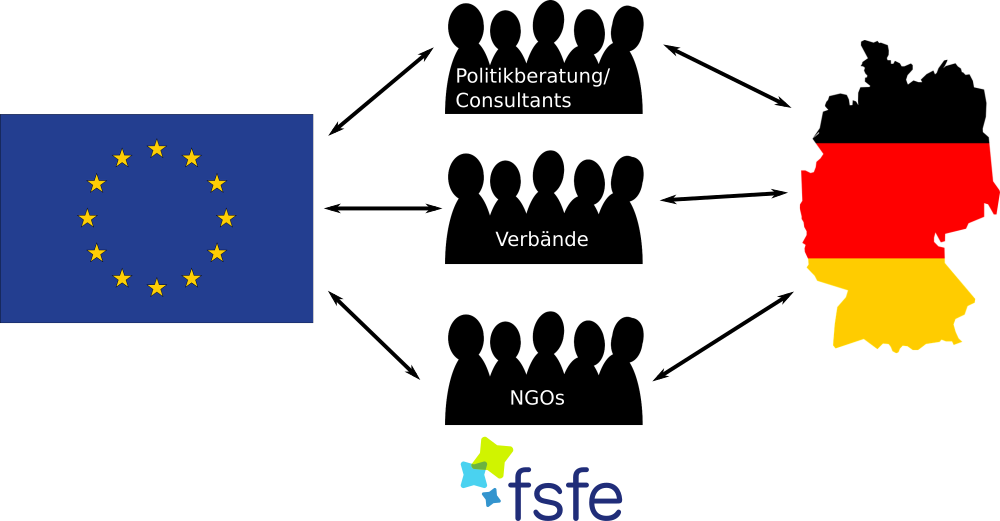
\includegraphics[width=\textwidth]{struktur}
	\centering
	\caption{Struktur des Lobbyismus}
	\label{fig:structure_image}
\end{figure}
In unsere heutigen Informationsgesellschaft ist klar zu verzeichnen, dass sich
die allgemeine Komplexität der Aufgaben, denen ein Staat, dessen Regierung und 
Bürger gegenüber stehen immens gestiegen ist und weiter wachsen wird.
Daraus entstehen folglich Probleme in der Entscheidungsfindung über Gesetze, da 
um solche durchschauen und verstehen zu können eine hohe Menge an Fachwissen 
nötig ist, die sich unmöglich eine einzelne Person aneignen kann. An der 
Schnittstelle, an welcher genau dieses Wissen der Exekutive zugeführt wird, 
setzt Interessenvertretung im allgemeinen an. Es wird im Prinzip mit Wissen 
bzw. Information Handel getrieben. Dies ist auch der Grund warum Leif und 
Speth\cite{LeifSpeth200312} Lobbyismus zu einer Branche erheben.

Leif und Speth führen weiterhin die Akteure des Lobbyismus an, unter 
welchen sich PR- und Image-Berater, Vertreter, Verbände, Wirtschaftsgruppen und 
NGOs befinden. Speziell die Verbände werden hier auch wissenschaftlich 
und vor allem im Kontext der Bundesrepublik Deutschland betrachtet.

Folglich wird dann auch auf Unterschiede zwischen Lobbyismus auf nationaler, 
europäischer oder Globaler Ebene geschlossen. Wie auf 
Abb.~\ref{fig:structure_image} 
deutlich wird, können z.B. die selben Lobbyingorganisationen sowohl auf 
Bundesebene als auch auf Europäischer ebene wirken. Allerdings müssen sie 
natürlich mit verschiedenen Regierungsformalismen und Bürokratien interagieren.

\subsection{Probleme}
Zu den geographischen Unterschieden gehört zusätzlich auch die Wahrnehmung bzw. 
Wertung des 
Lobbyismus als Hilfe bis hin zur Korruption. Nach Leif und Speth liegen die 
Gründe hierfür in den unterschiedlichen Ansichtsweisen bezüglich der jeweiligen 
in den Staaten vorherrschenden Demokratiemodelle. Die beiden Autoren führen 
hierbei den Pluralismus als Lobbyismus-akzeptierendes, wenn nicht sogar durch 
den Lobbyismus begründetes Modell an, welches dem Rousseau`schen Modell 
gegenübergestellt wird. Letzteres definiert Grundsätze der direkten Demokratie, 
in welcher es durch das Fehlen von 
''Vertretungskörperschaften``\cite{WikiIdentitaetstheorie} keinen 
Angriffspunkt, an dem Interessenvertretung wirken kann, gibt.

Es gibt allerdings auch modellunabhängige Kritikpunkte. Gesetzt dem Fall, man 
ist in der Lage wissenschaftlich abzuschätzen, wie viele Gesetze durch einwirken
von Interessengruppen und wie viele durch den Wahlprozess verabschiedet werden, 
könnte man zeigen das die Wahlen keinen großen Einfluss mehr auf die 
Entscheidungsfindung haben. Das Modell der Demokratie würde dadurch ad absurdum 
geführt werden. Es soll in dieser Arbeit kein ''Beweis`` für diese Aussage 
erbracht werden. Es ist jedoch davon auszugehen dass sie mittlerweile der 
Wahrheit entspricht.

% transparenzproblem und Asymmetrie der Interessenvertretungskraft
Es stellt sich daraus die Frage ob Lobbyismus in einem demokratischen Kontext 
existieren kann. Diese kann nur mit ''Ja`` beantwortet werden, wenn alle 
demokratiebedrohenden Faktoren behandelt und formalisiert werden. Das 
Kernproblem des Lobbyismus wurde bereits genannt. Die Interessenvertretung ist 
im Allgemein nicht gesetzlich geregelt, bzw. fehlt es ihr an ausreichend 
Transparenz um unbürokratisch zu verlaufen. Somit ist folglich nicht 
gewährleistet, 
dass auch Interessengruppen, welche finanziell nicht gut aufgestellt sind, die 
selbe Chance haben, ihre Ziele in den Politikprozess einzubringen. Beispiele 
wären hier z.B. Naturschutzvereine oder Menschenrechtsorganisationen, welche 
meistens nur begrenzt durch staatliche Förderungen und Spenden finanziert 
werden und somit nicht die selbe Wirksamkeit erzielen können wie eine 
Organisation die von einem Großkonzern gefördert wird.

\subsection{Formalisierungsversuche}
% Verhaltenskodex der Europäischen Kommession (Rechtsanwaltskanzleien)
Es existieren bereits Versuche, genau diese Probleme zu lösen. Der ``Rahmen für 
die Beziehungen zu Interessenvertretern''\cite{EuLobbyCodex} ist zum Beispiel 
ein Versuch der 
Europäischen Kommission, die Beeinflussung durch Akteure des Lobbyismus in 
geregelte Bahnen zu lenken. Es wird hier der Aufbau eines freiwilligen 
Registers angegangen, in welches sich Interessenvertreter eintragen können, 
insofern sie die Einhaltung des Codex beachten. Wer den Codex nicht beachtet 
würde öffentlich wieder aus dem Register ausgetragen werden. Somit kann sich 
hier eine Art Whitelist-Prinzip etablieren, in welchem - wenn es genügend 
Registereintragungen gibt - eine Nichteintragung gleichbedeutend mit einer 
schlechten ``Lobbyingbewertung'' wäre. Der Codex selbst regt zur Transparenz 
an, indem er die Offenlegung der Interessen, Klienten und 
Arbeitgeberorganisationen der Interessenvertreter fordert. Allerdings kann 
angenommen werden, dass Aktionen bei Nichteinhaltung des Codex nicht die 
mögliche Bestrafungswirksamkeit ausnutzen, wie folgendes Zitat zeigt:
\begin{displayquote}
``Im Falle eines mutmaßlichen Verstoßes kann jedermann bei der Kommission 
Beschwerde einlegen. Liegt der Kommission eine Beschwerde vor, wird sie vor der 
Einleitung eines förmlichen Verfahrens die betreffende Organisation bzw. 
Einrichtung um Klärung der Angelegenheit bitten und sie auffordern, die Regeln 
einzuhalten und gegebenenfalls falsche oder irreführende Informationen im 
Register zu berichtigen.''\cite{EuLobbyCodex}
\end{displayquote}
Ein weiterer Kritikpunkt an der Formulierung des Codex ist, dass er gezielt 
``Tätigkeiten im Zusammenhang mit Rechtsberatung''\cite{EuLobbyCodex} von der 
Pflicht sich in das Register einzutragen befreit. Diese werden jedoch in 
anderen Werken\cite{LeifSpeth200312} genau als Akteure der politischen 
Einflussnahme angeführt, was eine Art Hintertür bilden könnte.

% SEAP
Die Formalisierung der Aspekte des Lobbyismus geht aber auch von anderen 
Stellen aus. Hier angeführt sei die Society of European Affairs Professionals 
(SEAP), welche eine Organisation darstellt, die Schulungen für angehende 
Lobbyisten zur Verfügung stellt. Der wohl wichtigste Fakt ist jedoch hier, dass 
hier die Zugangs- bzw. Kontaktnetzwerke, welche die Akteure nutzen können 
gebündelt und festgehalten werden was wahrscheinlich effizienteres Lobbying 
ermöglicht. Es gibt noch mehr Organisationen wie die SEAP welche alle ihren 
eigenen Code of Conduct pflegen.\cite{2012lobbyists}

\subsection{Metalobbyismus}
Bei dem hier eingeführten Begriff des Metalobbyismus handelt es sich um ein 
spezielles Problem, was bei der bereits behandelten Schematisierung des 
Lobbyismus auftreten müsste. Dieses tritt genau dann auf wenn Unternehmen wie 
die SEAP wieder Interessenvertretung für ihre eigene Branche betreiben und 
genau dann wenn Lobbyismus eine eigenständige gewinnbringende Sparte im Markt 
bildet. Daraus könnte ein gewisser Selbsterhaltungsmechanismus der 
Lobbyingorganisationen entstehen welcher diesen wiederum zu gute kommt und dazu 
führen könnte dass sich diese Organisationen nach und nach von ihrem 
ursprünglichen Aufgabengebiet ablösen.

Es ist somit ein ausreichender Grundstock an Informationen über das Thema 
Lobbyismus gelegt um im folgenden genau zu klären, inwiefern die FSFE Lobbying 
betreibt.

\newpage
\section{Die FSFE als Lobbyorganisation}
\epigraph{Politischen Wandel und politische Meinungsbildung zugunsten Freier 
Software zu beeinflussen ist sicherlich ein wichtiger Aspekt unserer 
Arbeit}{George Greve}

% Lobbydef aufFSFE  anwenden und dabei FSFE Weiter erklären
% Aussagen von Greve Benutzen \cite{PLGreveInterView}

\subsection{Wirken der FSFE - Kampagnen}
Die Arbeit der FSFE findet unter anderem in unterschiedlichen Kampagnen statt, 
welche die Grundlage für die meinungsbildende Wirkung der Organisation stellt.

% indirekter Lobbyismus über z.B. FFII
% Weltgipfel der Vereinten Nationen \cite{PLGreveInterView}
% FFII zugearbeitet \cite{PLGreveInterView}
% Secureboot (FSFE website)


\begin{itemize*}
    \item Secureboot anschauen -- Einflusssicherungsversuch von anderen
    Unternehmen
\end{itemize*}

\begin{itemize*}

% indirekten Lobbyismus für FInanzierung wieder aufgreifen
% Geldgeber hat Macht oder Pflicht? \cite{PLGreveInterView} S2-23
\item Finanzierung I
\item Finanzierung II
\item welcher Einfluss ergibt sich dadurch
\item welche Unternehmen haben wie Einfluss auf die FSFE?
\end{itemize*}

\section{Unterschied zu anderen Lobbyingarten}
\begin{itemize*}
\item Pharmalobby \cite{BeckLobbyGesundwe}
\item Agrar-Lobbying
\item IT-Lobby
\item struktureller Vergleich
\item finanzieller Vergleich
\item regionaler Vergleich (Weltweit, Europa, Landesebene)
\item Transparenz, Transparenz, Transparenz!!!
\end{itemize*}

\section{Schluss}
\begin{itemize*}
\item Lobbying als natürlicher Vorgang (Eigene These)
\item Klare Unterschiede Intensität
\item Wahlpoolidee
\end{itemize*}

\newpage
\bibliography{refs}
\bibliographystyle{plain}
\todo[inline]{Bibtexvorlage der Uni benutzen}
\todo[inline]{Unterlagen zuhause checken}

\listoftodos

\end{document}
